The basic representation of a complex zonotope is a linear combination
of complex valued vectors with complex combining coefficients whose
absolute value is bounded by unity.  This is a generalization of the
representation of a simple zonotope given in Definition~\ref{defn:rztope} of
previous chapter to the space of complex numbers.  However, the real
projection of a complex zonotope is expressive because it can
represent some non-polyhedral sets in addition to the polyhedral
zonotopes, which we shall discuss later.
%
\begin{definition}[Complex zonotope]
Let $\ptemp\in\mat{m}{n}{\compnums}$ be a complex valued matrix
whose columns are called {\it generators} and $\cen\in\compnums^n$ be a
complex valued vector called the {\it center}.  The following is the
representation of a
complex zonotope.
%
\begin{equation}
\cztope{\ptemp}{\cen} := \set{\ptemp\zeta+\cen:~\zeta\in\compnums^m,~\infnorm{\zeta}\leq 1}.
\end{equation}
%
\end{definition}
%
{\it Shape of complex zonotope:} The real projection of a complex
zonotope can represent non-polyhedral sets, which can be Minkowski sum
of line segments as well as some ellipsoids.  Therefore, complex
zonotopes are more expressive than real zonotopes.  An example of such
a non-polyhedral complex zonotope projection in real space is
illustrated with Figure~\ref{fig:cz}, where the generators are
$\ptemp=\lt(\begin{array}{lll}(1+2i) & 1 & (2+i)\\(1-2i) & 1 &
(2-i)\end{array}\rt)$ and the center is the origin.  Furthermore,
complex zonotopes are different from polynomial zonotopes.  While a
polynomial zonotope is a polynomial function of real valued intervals,
a complex zonotope is a Minkowski sum of \emph{linearly transformed
transformed circles} in the the complex plane.  A complex zonotope is
symmetric around the center.  To see this, consider a point in a
complex zonotope centered at the origin, written as $y=\ptemp\zeta$
where $\ptemp$ defines the generator set and $\zeta$ is the vector of
combining coefficients.  Since, $\infnorm{-\zeta}=\infnorm{\zeta}\leq
1$, so $-y=\ptemp(-\zeta)$ also belongs to the complex zonotope.
%
\begin{figure}
\centering
\captionsetup{justification=centering}
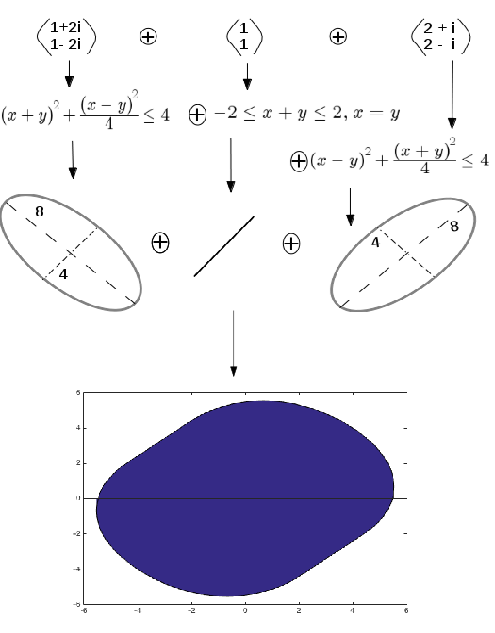
\includegraphics[scale=0.43]{fig/cznew.png}
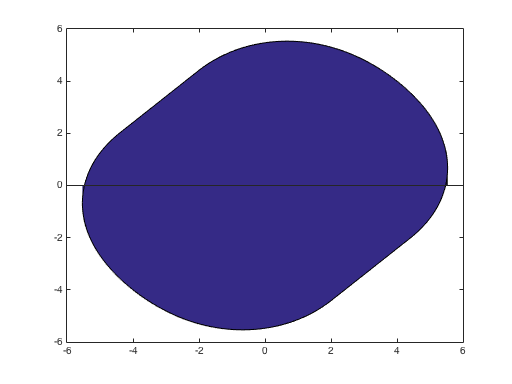
\includegraphics[scale=0.5]{fig/CZhull.png}
\caption{Real projection of a complex zonotope as\\ Minkowski sum of 2 ellipses and 1 line segment }        
\label{fig:cz}
\end{figure}
%
A motivation for extending simple zonotopes to complex zonotopes is
that a complex zonotope with its generators as the complex
eigenvectors of a discrete time linear system will be a positively
invariant if the complex eigenvalues corresponding to the generators
are bounded within unity in their absolute values.  This property is
explained mathematically in the following proposition.
%
\begin{proposition}[Eigenstructure based invariance]~\label{lem:eig-invariance}
Let us consider $\ptemp\in\mat{n}{n}{\compnums}$ consists
of the complex eigenvectors of a matrix $A\in\mat{n}{n}{\reals}$ as
its column vectors and $\mu\in\compnums^n$ be the vector of complex
eigenvalues, i.e., $A\ptemp
= \ptemp\diagonal{\mu}$.  Then \[A\lt(\cztope{\ptemp}{0}\rt)
= \cztope{\ptemp\diagonal{\mu}}{0}.\] If
$\infnorm{\mu}\leq 1$, then
$A\lt(\rztope{\ptemp}{0}\rt)\subseteq \rztope{\ptemp}{0}$.
\end{proposition}
% 
\begin{proof}
We derive
  %
\begin{align*}
& A\lt(\cztope{\ptemp}{0}\rt) =
A\set{\ptemp\zeta:~\zeta\in\compnums^n,\infnorm{\zeta}\leq 1}\\
& =\set{A\ptemp\zeta:~\zeta\in\compnums^n,\infnorm{\zeta}\leq 1}
= \cztope{A\ptemp}{0}=\cztope{\ptemp\diagonal{\mu}}{0}.
\end{align*}
%
which proves the first part of the
Proposition.

For the second part, we are given that $\infnorm{\mu}\leq 1$.
Consider a point
%
\begin{align*}
  & y\in A\cztope{\ptemp}{0}=\cztope{\ptemp\diagonal{\mu}}{0}~~\text{where}\\
  &y = \ptemp\diagonal{\mu}\delta:\infnorm{\delta}\leq
1.
\end{align*}
%
Let $\zeta = \diagonal{\mu}\delta$. Then $\infnorm{\zeta} \leq
\infnorm{\mu}\infnorm{\delta} \leq 1$.  So,
%
\begin{align*}
  & y=\ptemp\zeta~~\text{ where }~
  \infnorm{\zeta}\leq 1.
\end{align*}
%
So, we get $y\in \cztope{\ptemp}{0}$.  As this is true for all
$y\in\cztope{\ptemp}{0}$, we have
$A\lt(\cztope{\ptemp}{0}\rt)\subseteq
\cztope{\ptemp}{0}$ when $\infnorm{\mu}\leq 1$.
\end{proof}
%



If we add more generators to the above representation of a complex
zonotope, it would increase the size of the complex zonotope.
Therefore, we can not find better approximations of a given set by
only adding more generators to the complex zonotope.  Moreover, adding a
generator can violate positive invariance, as shown in
Figure~\ref{todo}.  Alternatively, to refine a complex zonotope, we
can adjust the magnitude of contribution of each generator to the size
of the set while also preserving the positive
invariance.  This way can also add more generators to refine the
complex zonotope, by adjusting the
magnitude of contribution of each generator.

In order to conveniently perform algebraic manipulations on the
magnitude of each generator, we can explicitly specify values
proportional to their magnitudes as part of the set representation.
In this regard, we introduce a {\it template complex zonotope}
representation, where the magnitude of each combining coefficient is
bounded in its absolute value by a positive real, called a {\it
  scaling factor}.  We call the matrix whose column vectors generate a
template complex zonotope as a {\it template}.  This representation is
similar in spirit to the known template based set
representations~\cite{todo} in abstract interpretation, where for some
fixed template, subsets
of metric spaces are mapped to points in a lattice.  In the case of a
template complex zonotope, for a fixed template, subsets of the
complex vector space can be mapped to the {\it scaling factors}.
%
\begin{definition}[Template complex zonotope]
Let us consider ${\ptemp\in\mat{n}{m}{\compnums}}$ called the template,
${\sfact\in\reals^m_{\geq 0}}$ called scaling factors and
${\cen\in\compnums^n}$ called the center.  Then the following is a template
complex zonotope.
%
\begin{equation}
\tcztope{\ptemp}{\cen}{\sfact}
= \set{\ptemp\zeta+\cen:~\absolute{\zeta_i}\leq \sfact_i~\forall
i\in\set{1,...,m}}.
\end{equation}
\end{definition}
In further discussion, we use the term {\it representation size} of a
template complex zonotope to refer to the size of the template matrix.
In the rest of this chapter, we consider the following notation,
unless otherwise specified.
%
\[
\ptemp\in\mat{n}{m}{\compnums},~~\cen\in\compnums^n,~~\sfact\in\reals^m_{\geq 0}.
\]
%
A template complex zonotope can be converted to the basic
representation of the complex zonotope by multiplying the diagonal
matrix of scaling factors to the template.  This is described in the
following lemma.
%
\begin{lemma}[Normalization]~\label{lem:normalization}
Let us consider ${\mu\in\compnums^m}$.
%
\begin{align*}
\text{Then}\hspace{3em}&\tcztope{\ptemp\diagonal{\mu}}{\cen}{\sfact}=\tcztope{\ptemp}{\cen}{\diagonal{\absolute{\mu}}\sfact}.~\numberthis\label{eqn:normalization}\\
\text{Therefore},\hspace{3em} & \tcztope{\ptemp}{\cen}{\sfact}=\cztope{\ptemp\diagonal{\sfact}}{\cen}.
\end{align*}
%
\end{lemma}
%
\begin{proof}
Consider a point $x\in\tcztope{\ptemp\diagonal{\mu}}{\cen}{\sfact}$,
where
%
\[
x=\cen+\ptemp\diagonal{\mu}\zeta:\absolute{\zeta}\leq\sfact.
\]
%
Let $\zeta^\pr=\diagonal{\mu}\zeta$.  Then, $x=c+\ptemp\zeta^\pr$.
We get
%
\[
\absolute{\zeta^\pr}=\diagonal{\absolute{\mu}}\absolute{\zeta}\leq\diagonal{\absolute{\mu}}\sfact.
\]

Therefore, ${x\in\tcztope{\ptemp}{\cen}{\diagonal{\mu}\sfact}}$.  This
means,
%
\[
\tcztope{\ptemp\diagonal{\mu}}{\cen}{\sfact}\subseteq\tcztope{\ptemp}{\cen}{\diagonal{\absolute{\mu}}\sfact}
\]
%
Next consider a point
$y\in\tcztope{\ptemp}{\cen}{\diagonal{\absolute{\mu}\sfact}}$ where
%
\[
y=\cen+\ptemp\epsilon:~\absolute{\epsilon}\leq
\diagonal{\absolute{\mu}}\sfact.
\]
%
Let us consider $\epsilon^\pr\in\compnums^m$, such that
%
\[\forall i\in\set{1,...,m},~~
\epsilon_i=\left\{
\begin{array}{l}
\frac{\epsilon_i}{\mu_i}~\text{if}~\mu_i\neq 0\\
0~\text{if}~\mu_i=0.
\end{array}
\right.
\]
%
We shall show that $\epsilon=\epsilon^\pr\diagonal{\mu}$, i.e., for
any $i\in\set{1,...,m}$, $\epsilon_i=\epsilon^\pr_i\mu_i$.  We prove
it in the following two cases.
\begin{enumerate}
\item Let us consider $\epsilon_i\neq 0$.  As
$\absolute{\epsilon}\leq\absolute{\diagonal{\mu_i}}\sfact$, so
  $\mu_i\neq 0$.  Therefore,
  \[
  \epsilon_i=\frac{\epsilon_i}{\mu_i}\mu_i=\epsilon^\pr_i\mu_i.
  \]
\item Let us consider $\epsilon_i=0$.  As
$\absolute{\epsilon}\leq\absolute{\diagonal{\mu_i}}\sfact$, so $\mu_i=
  0$.  This implies
  \[
  0=\epsilon=\epsilon^\pr_i\times
  0=\epsilon^\pr_i\mu_i.
  \]
  %
\end{enumerate}
%
So, we get $y=\cen+\ptemp\diagonal{\mu_i}\epsilon^\pr$.  By the definition of
$\epsilon^\pr$, we get
%
\[\forall i\in\set{1,...,m}~~
\absolute{\epsilon^\pr_i}\leq
\left\{
\begin{array}{l}
\absolute{\frac{\epsilon_i}{\mu_i}}\leq\frac{\absolute{\mu_i}\sfact_i}{\absolute{\mu_i}}=\sfact_i~\text{if}~\mu_i\neq
0\\
0~\text{if}~\mu_i=0
\end{array}
\right.
\]
%
Therefore, $\absolute{\epsilon^\pr}\leq\sfact$.  So,
$y\in\tcztope{\ptemp\diagonal{\mu}}{\cen}{\sfact}$.  Therefore,
%
\[
\tcztope{\ptemp}{\cen}{\diagonal{\absolute{\mu}}\sfact}\subseteq\tcztope{\ptemp\diagonal{\mu}}{\cen}{\sfact}.
\]
%
Combining the previous two conclusions, we get
Equation~\ref{eqn:normalization}.

By definition,
%
\begin{align*}
& \cztope{\ptemp\diagonal{\sfact}}{\cen}=\tcztope{\ptemp\diagonal{\sfact}}{\cen}{\repmat{1}{m}{1}}\\
& \%\%~~\text{by Equation~\ref{eqn:normalization}}\\
& =\tcztope{\ptemp}{\cen}{\diagonal{{\sfact}}\repmat{1}{m}{1}}=\tcz{\ptemp}{\cen}{\sfact}.~\hspace{3em}\qedhere
\end{align*}
%
\end{proof}
%
